%% This is an example first chapter.  You should put chapter/appendix that you
%% write into a separate file, and add a line \include{yourfilename} to
%% main.tex, where `yourfilename.tex' is the name of the chapter/appendix file.
%% You can process specific files by typing their names in at the 
%% \files=
%% prompt when you run the file main.tex through LaTeX.
\chapter{1. Introduction}

\section{Overview}
\justify
Technology and its products influences the public norm, which then will affect the tools; both have a mutual dependence.
This thesis positions a novel tool for civic engagement within this loop of society and technology influencing each other. 

\begin{figure}[!htb]
 	
\includegraphics[width=\textwidth]{chapters/1/fig/hearings.png}               
 	 \caption[diagram: community hearings]{The pyramid divided into two parts; The top portion includes the Planners, Governors, and Stakeholders, and the \textbf{rest}. Public hearings are communication tools to let the top know the bottom. The arrow pointing to the black border indicating it changes the infrastructure, which is the boarder of the build environment and the natural environment.}
  	\label{fig:hearings}
\end{figure}

Traditionally the urban planning process accommodates public feedback through community hearings for voicing concerns from the community. The planners, government, and stakeholders will interpret the input, and plan and execute interventions that consider citizen feedback. We can think of this model as a technology to accommodate feedback once cities became too large for governance via direct democracy.

\begin{figure}[!htb]
 	
\includegraphics[width=\textwidth]{chapters/1/fig/community_engagement.png}               
 	 \caption[externalized proposal]{Demand from both the planners (wicked problem \cite{churchman1967guest}) and the community (evidence of urbanization leads to democratization \cite{woolley2010evidence} )to externalize the proposal (rectangle with P). Now citizens can provide feedback and co-design the interventions. This is the typical diagram for today's community engagement. The planners are still proposing the plans which are the primary generator of solutions.}
  	\label{fig:spin_margin}
\end{figure}

Urbanisation occurs and as cities become more dense, public demand for transparent planning increases, which results the plan to be externalized for scrutiny by the community. This increased interest in urban planning, especially transportation planning, points to the opportunity for new tools to better serve public needs.

In addition, new tools that leverage pervasive mobile communications have been developed to collect data in the form of reports and claims. These applications can be categorized as 'structured' / 'unstructured'. The majority of these applications solicit unstructured feedback, making them useful for general comments, but limiting their utility for actionable information.

These tools are mainly used for analysing the current situation, distinct from integrating (synthesis) it to one executable plan. Designers and architects have been continuously arguing that the process of analysis and synthesis should be close as possible to design properly. This mainly comes from the difference in objectives because designers and architects focuses on the integration plans rather than to provide insights. The disjoint of analysis and synthesis is one reason of failing design, since essential to the feedback process. 
Because the synthetic process in planning required domain knowledge and was hard and notably slow, the community had limited exposure to this phase of the realization of the program. Thus, community engagement processes do not have a clear distinction between the two major phases of design.

\begin{figure}[!htb]
 	
\includegraphics[width=\textwidth]{chapters/1/fig/cityscope.png}               
 	 \caption[diagram: cityscope model]{The cityscope model covers the analysis through the prioritization phase. Apart from the visualization and tangible interface, it is a tool for iterating the analytical phase and synthetical phase. Note the arrow from Planners to the Plan is approval, which the plan generation is a collective collaboration from the whole community.}
  	\label{fig:diagram_cityscope}
\end{figure}

New tools have been focusing on supporting specific parts of the process, but are fragmented.
As they become mature, there is potential to have them integrated so the transition of the analytical and synthetic phase will be easier. Resulting to have more rapid iteration loops.

This thesis looks at a specific topic in urban planning: making cities more accessible to bicycles. The tool - bikebump - that allows users to passively report problems with urban infrastructure, then invites them to actively participate in planning processes to improve the urban environment. Having an integrated platform though the data collection and plan proposal is what makes this attempt novel.

\begin{figure}[!htb]
 	
\includegraphics[width=\textwidth]{chapters/1/fig/bikebump.png}               
 	 \caption[diagram: bikebump]{The thesis investigates for a integrated tool that starts with the data collection though prioritisation.}
  	\label{fig:diagram_bikebump}
\end{figure}

The evolution of technological tools for urban planning and their relationship to public demands will be explored in the background section, before introducing the BikeBump intervention. 

\begin{figure*}[!htb]

\includegraphics[width=\textwidth]{chapters/1/fig/proposed_process.png}               
 	 \caption[proposed method]{The proposed method using bikebump trying to fit the current system. The Transportation Improvement Program (TIP) is a federal requirement for each state to compile a list of executable improvements regarding transportation issues. The top of the pyramid from the previous diagrams is the Metropolitan Planning Organization and the Mayor (city CEO), given a roll of approval (which is no different from another single vote) and metric modification and engineering of plans. The improvement plans that was generated and prioritized by bikebump will undergo one last process of being approved by the Transportation Advisory Council which also tied to a public hearing.}
  	\label{fig:proposed}
\end{figure*}

Figure \ref{fig:proposed} shows a possible method form of approving bike lane improvement using this approach. There are two major differences compared to the method that is currently conducted through the United States. One, the box has inputs in two different directions from the community indicating the data collection and proposal. This is the core of this tool integrating the analytical phase and synthetic phase in one platform. Two, the planners (Metropolitan Planning Organization) and the authority (city CEO) will have a meta roll on approving and modifying the metrics to align with the long running plans. The comparison of the methodology will discussed in the Design and Implementation.
In chapter xx, I will introduce the tools and methods used for developing this web-based application, and the procedure of how it will work. The application is a web based application that runs in android devices using the standard Chrome browser.

Figure \ref{fig:how} shows the procedure of the user experience. The application has access to the phone's microphone and can detect the ring of a bicycle bell throughout the commute, saving a short sound clip of the moment before the bell ring. The sound data, the number of consecutive rings and geolocation will sent to the server for further analysis. The data will be mapped to a web browser interface that others would be able to observe. After the commute, the application will show a set binary choice questions and suggestions to ask how the situation on the street where the bell was sounded could be improved.

\begin{figure}[!htb]
 	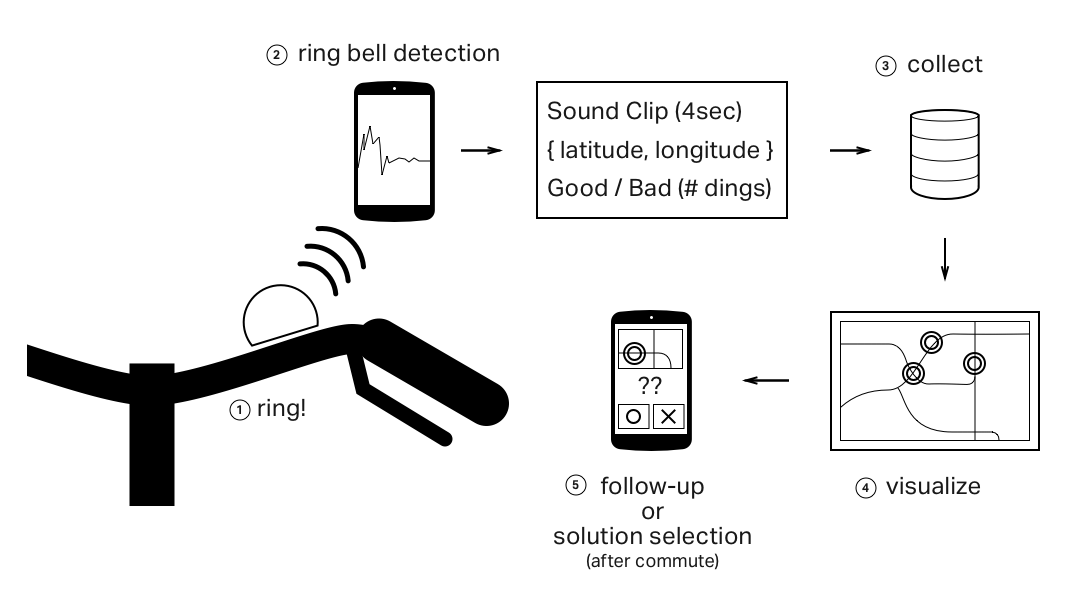
\includegraphics[width=\textwidth]{chapters/1/fig/how_it_works.png}               
 	 \caption[how bike bump works]{
 	 The flow of user interaction
 	 \begin{enumerate}
 	 \item the user rings bell if there is something worth reporting (a DING). Simple protocol of single ding indicating ``unsafe/dangerous'' and double ding indicating ``safe/pleasant''
 	 \item Smartphone detecting the frequency of the bell
 	 \item Geolocation, ``dangerous/pleasant'' value, and sound clip sent to database
 	 \item visualised to map
 	 \item user provides complementary information about the DING. Users can also propose a improvement plan by selecting a solution and the road.
 	 \end{enumerate}}
  	\label{fig:how}
\end{figure}

\section{Contribution}
The main contributions of the thesis are to connect citizens into the urban planning process through a novel technological solution. By harnessing feedback from individual bicyclists, the tool opens the urban planning process beyond mayors, professional planners and includes average citizens and collectively architect the physical environment surrounding use.
It may also help the planning side, which traditionally consist urban planners, mayors, and other stakeholders to understand the residents demand. In addition, the schema for the new urban planning support tool will externalize the process plan analysis and synthesis, which is often tacit knowledge within the planners.
The study proposes a bi-directional communication method to connect the top and bottom of the process.
